\documentclass[letterpaper,journal]{IEEEtran}
\usepackage{amsmath,amssymb}
\usepackage{booktabs}
\usepackage{graphicx}
\usepackage{url}
\usepackage{cite}
\usepackage{geometry}
\usepackage{fancyhdr}

\geometry{
    letterpaper,
    top=26mm,
    headheight=14pt,
    bottom=20mm,
    left=20mm,
    right=20mm
}

\graphicspath{{figures/}}

\fancypagestyle{courseproject}{%
    \fancyhf{}%
    \fancyhead[L]{\small ENGG 5402 Advanced Robotics}%
    \fancyhead[R]{\small Final Project Group 11}%
    \fancyfoot[C]{\small\thepage}%
    \renewcommand{\headrulewidth}{0pt}%
}

\begin{document}
\pagestyle{courseproject}

\title{UR5e Navigation by Touch Among Fixed Obstacles: A Comparison of A* and MDP Planning}

\author{To Pak Kiu Katy, Rezaeichiyaneh Pariya, Hong Yue, Lee Chun Long}%

\maketitle
\thispagestyle{courseproject}

\begin{abstract}
We compare A* and Markov decision process (MDP) planning for a UR5e probe that navigates a flat workspace by touch. Four fixed boxes block the direct route. With a rough map, both planners start with occupancy probabilities based on box positions that may be off by up to 5~cm. With unknown boxes, both use the same recovery routine. After contact, the probe moves along the box face in 1, 3, or 5~cm steps. It attempts a 1~cm move perpendicular to the face after each step and stops if it makes contact. The planner takes over when the check is clear. Each strategy was simulated once, and all eight runs reached the goal. With the rough map, the MDP was fastest (93.44~s) and made no contacts. With unknown boxes, A* was fastest at 5~cm (96.80~s, four contacts), and the MDP was fastest at 3~cm (251.10~s, 31 contacts). At 5~cm, the MDP made fewer contacts (25) and took longer because it traveled farther.

\end{abstract}

\begin{IEEEkeywords}
Tactile navigation, UR5e, occupancy grid, A*, Markov decision process, contact recovery.
\end{IEEEkeywords}

\section{Introduction}

A probe that navigates by touch learns which cells are clear or blocked as it moves. With an inaccurate map, a short route can lead to repeated stops and retreats. A planner can use occupancy probabilities to choose a longer route with fewer interruptions. We compare two planners on the same box layout, first with a rough map and then with no box information. We measure goal completion, contact count, completed route length, total probe travel, and simulated execution time.

\section{Related Work}

A* ranks grid cells using the cost of reaching each cell and an estimate of the cost from that cell to the goal \cite{hart}. When new observations change the map, methods such as D* Lite can reuse earlier search results \cite{koenig2002dstar}. An occupancy grid assigns each cell a probability of being blocked \cite{elfes1989occupancy,thrun}.

In Bug algorithms, a robot moves toward the goal and follows an obstacle's boundary when it encounters one \cite{lumelsky1987path}. Robot arms can also use touch to estimate the position and orientation of objects with known shapes \cite{petrovskaya2011touch}. Both planners use the same kind of grid observations in each scenario. They also use the same box-edge routine when box locations and sizes are unknown.

An MDP uses probabilities and rewards to describe the possible outcomes of each action \cite{puterman}. A partially observable MDP plans using a probability distribution over possible states, so it can account for what a new observation might reveal \cite{kaelbling1998pomdp}. Our MDP uses the probe's current grid cell as its state. It replans on the updated grid as new observations arrive.

\section{Workspace and Occupancy Model}

\subsection{Workspace and fixed obstacles}

The workspace is a $60\times40$~cm rectangle divided into $1\times1$~cm grid cells. We label each cell by its row and column $(r,c)$. Its center is $(c+0.5,r+0.5)$ in table coordinates. The probe starts at $s_0=(20,3)$ and aims for $s_g=(20,56)$. The direct route crosses boxes B1, B2, B3, and B4 in that order. The closest pair of actual boxes has a 3~cm gap between its edges. The boxes stay fixed in both scenarios. Table~\ref{tab:layout} lists the box sizes and positions, and Fig.~\ref{fig:layout} shows the layout.

\begin{table}[t]
\centering
\caption{Box sizes and lower-left corners in cm.}
\label{tab:layout}
\begin{tabular}{@{}lccc@{}}
\toprule
Box & Width $\times$ height & Nominal $(x,y)$ & Actual $(x,y)$\\
\midrule
B1 & $10\times5$ & $(5,20)$ & $(8,19)$\\
B2 & $11\times12$ & $(26,11)$ & $(23,10)$\\
B3 & $6\times6$ & $(37,23)$ & $(37,19)$\\
B4 & $8\times11$ & $(46,13)$ & $(46,13)$\\
\bottomrule
\end{tabular}
\end{table}

\begin{figure*}[t]
\centering
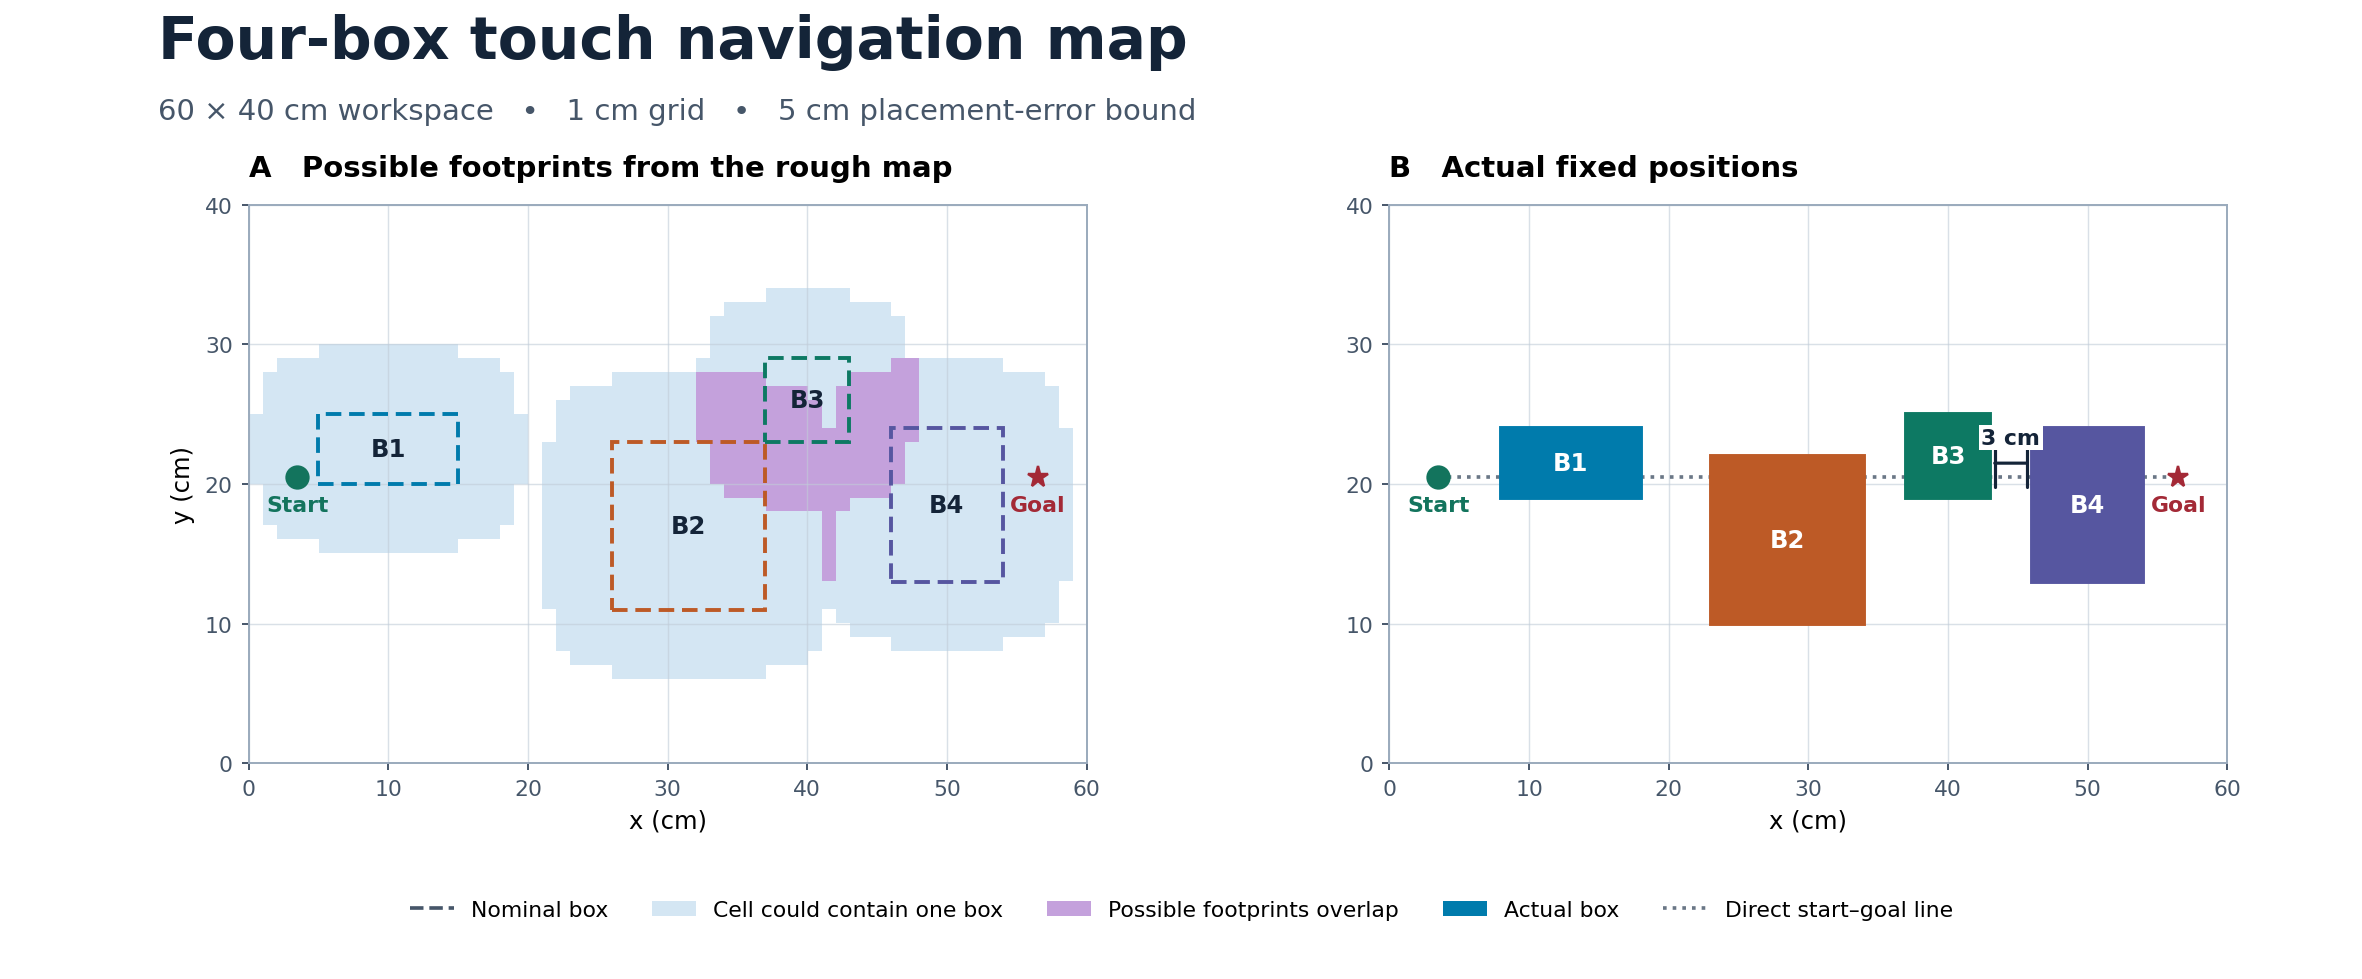
\includegraphics[width=.94\textwidth,height=.225\textheight,keepaspectratio]{four_box_touch_navigation_map.png}
\caption{Nominal box outlines and possible footprints under the rough prior (left), and the fixed boxes used for collision detection (right). The dotted line shows the direct route from start to goal.}
\label{fig:layout}
\end{figure*}

\subsection{Starting occupancy probabilities}

Let $B_i^0$ be the area that box $i$ covers in the rough map. The model shifts each box independently, with every offset in the following grid disk equally likely.

\begin{equation}
 \mathcal{D}_5=\{(u,v)\in\mathbb{Z}^2:u^2+v^2\le 25\},\quad
 |\mathcal{D}_5|=81.
\end{equation}

For any cell $z$, the occupancy probabilities are

\begin{align}
 p_i(z)&=\frac{1}{81}\sum_{\delta\in\mathcal{D}_5}
 \mathbf{1}\{z\in B_i^0+\delta\},\\
 p_0(z)&=1-\prod_{i=1}^4[1-p_i(z)].
\end{align}

None of the 6,561 offset pairs make B1 and B2 overlap. For B3 and B4, 653 of the 6,561 pairs (9.95\%) produce an overlap. The actual boxes are at least 3~cm apart. When the boxes are unknown, each cell starts with a 0.05 probability of being occupied. The start cell is marked clear. Figure~\ref{fig:prior} shows both maps.

\begin{figure*}[t]
\centering
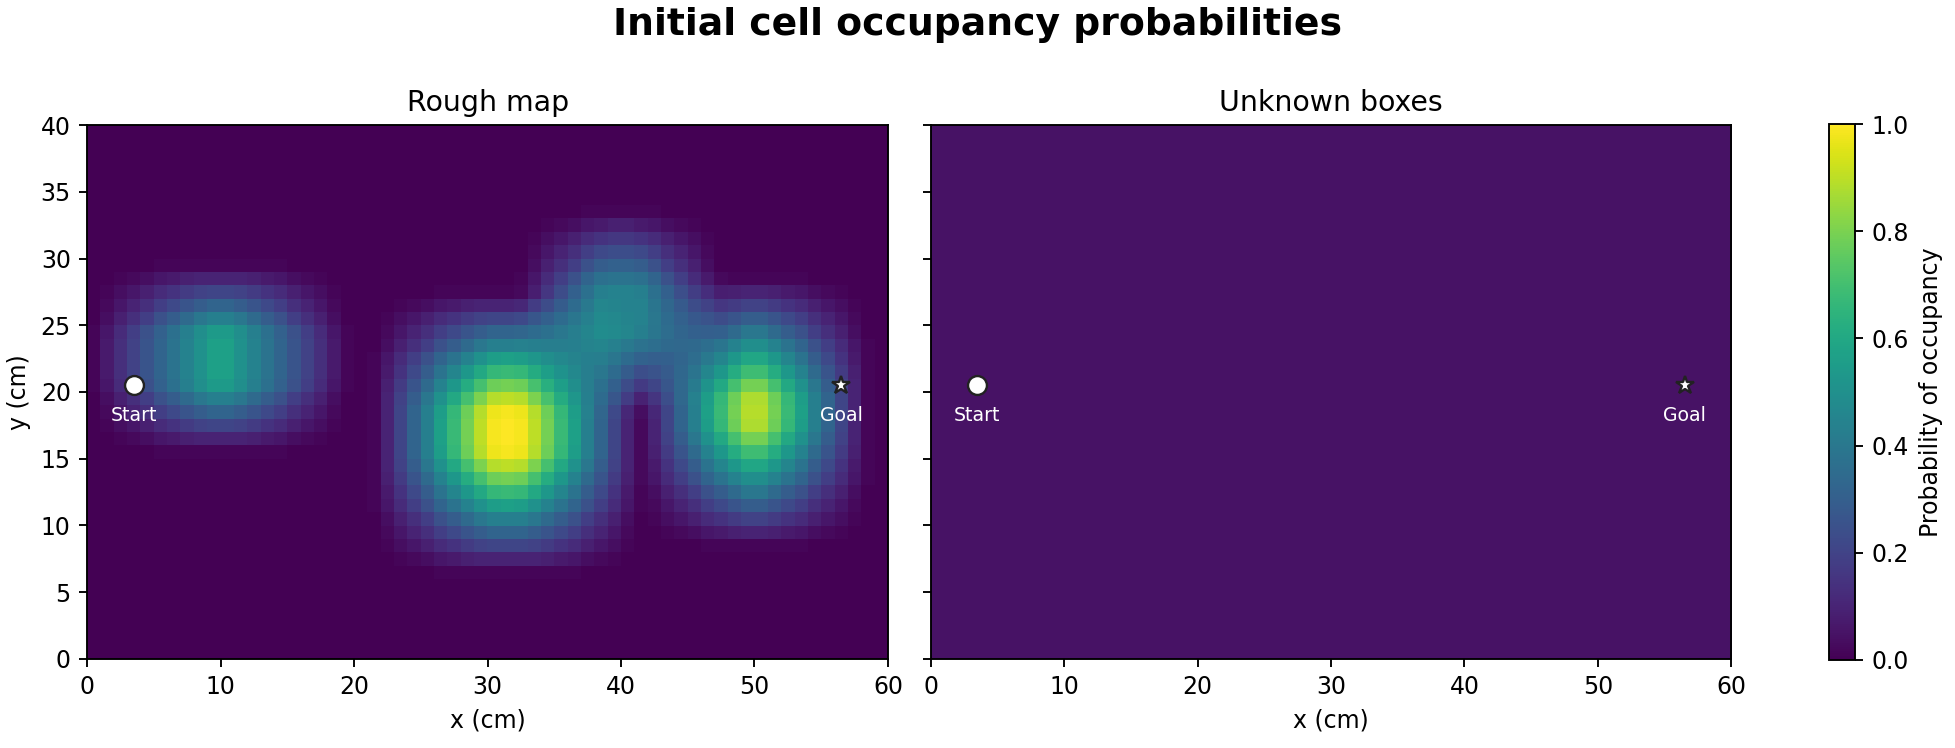
\includegraphics[width=.9\textwidth,height=.215\textheight,keepaspectratio]{occupancy_probability_maps.png}
\caption{Starting probability that each cell is occupied. In the rough map, cells near the estimated box locations are more likely to be occupied. In the unknown-box case, all cells except the start use the same probability.}
\label{fig:prior}
\end{figure*}

\section{Navigation Strategies}

\subsection{Actions and box-edge following}

The grid directions are $\mathcal U=\{-1,0,1\}^2\setminus\{(0,0)\}$. With the rough map, the planner can move one cell horizontally, vertically, or diagonally. Horizontal and vertical moves cover 1~cm, and diagonal moves cover $\sqrt2$~cm. A diagonal move sweeps the destination and both neighboring side cells. Contact with a box in any of these cells interrupts the move. With unknown boxes, ordinary moves are 1~cm horizontally or vertically.

When a horizontal or vertical move hits an unknown box, the probe stops and returns to the cell where the move began. Let $\mathbf n$ be the unit grid direction in which the probe approached the box, and let $\mathbf t$ be a perpendicular unit grid direction along its face. The probe chooses the direction along the face using the goal's position along the tangent axis, with a fixed direction when the tangent coordinates are equal. For a step of $D\in\{1,3,5\}$~cm along the edge, the two target cells are

\begin{equation}
 s_{\parallel}=s+D\mathbf t,\qquad
 s_{\mathrm{check}}=s_{\parallel}+\mathbf n ,
 \label{eq:edge_targets}
\end{equation}

where grid cells are 1~cm apart and the workspace boundary limits the step along the edge. The probe checks for contact throughout every move. After a clear edge step, it attempts a 1~cm move perpendicular to the edge. If the check hits, the probe returns to $s_{\parallel}$, takes another edge step, and checks again. If the check is clear, the probe reaches $s_{\mathrm{check}}$ and returns control to the planner. The routine uses no box-size information. A blocked edge step or the workspace boundary can make the probe reverse direction once before planning resumes.

Both planners update cells using

\begin{equation}
 p_{t+1}(z)=
 \begin{cases}
 1,&z\text{ is the reported contact cell},\\
 0,&z\text{ is observed clear},\\
 p_t(z),&\text{otherwise}.
 \end{cases}
\end{equation}

If a move spans several cells and hits a box, the simulator can mark the cells it passed through as clear before recording the hit. Each check that hits the box counts as one contact.

\subsection{A*}

A* initially treats cells with $p_t(z)>0.5$ as blocked. It allows a move if every cell along the move has an occupancy probability of 0.5 or less. A* ranks cells by $f(s)=g(s)+h(s)$, where $g(s)$ is the path length so far and $h(s)$ estimates the remaining distance. With the rough map, A* uses the octile heuristic to account for diagonal moves.

\begin{equation}
 h(s)=\max(\Delta r,\Delta c)+(\sqrt2-1)\min(\Delta r,\Delta c),
\end{equation}

where $\Delta r$ and $\Delta c$ are the absolute row and column differences to the goal. With the rough map, A* keeps its current path until it needs to replan. If it finds no path with the 0.5 threshold, it tries again while blocking only confirmed occupied cells. With unknown boxes, A* searches from the current cell for each ordinary move. It uses straight-line distance as its heuristic and prefers fewer moves when path lengths are equal.

\subsection{MDP planner}

Let $\mathcal W(s,a)$ be the set of cells that the probe passes through when it takes action $a$ from cell $s$. The MDP estimates the probability that the move is clear using

\begin{equation}
 q_t(s,a)=\prod_{z\in\mathcal W(s,a)}[1-p_t(z)].
\end{equation}

This estimate treats each cell's occupancy as independent. A successful move has a cost of $\ell(a)$. A contact adds a penalty of $C=20$, and the probe returns to the cell where it started the move. The discount factor is $\gamma=0.99$, and the value at the goal is $V(s_g)=100$. The Bellman equations are

\begin{align}
 V(s)&=\max_a Q(s,a),\\
 Q(s,a)&=q_t(s,a)[-\ell(a)+\gamma V(s')]\notag\\
 &\quad+[1-q_t(s,a)][-C+\gamma V(s)].
\end{align}

A contact returns the probe to the same cell. Rearranging the Bellman equations removes this self-loop from the value iteration update:

\begin{equation}
 V(s)=\max_a\frac{
 q_t(s,a)[-\ell(a)+\gamma V(s')]
 -[1-q_t(s,a)]C}{1-\gamma[1-q_t(s,a)]}.
\end{equation}

With the rough map, the MDP replans when occupancy changes. With unknown boxes, it plans 1~cm horizontal and vertical moves and starts each round of value iteration with the previous value estimates. The Bellman update treats each contact as a penalty followed by a return to the same cell. The box-edge routine in \eqref{eq:edge_targets} runs separately, so the update does not include the cost of moving along the edge or making the extra checks.

\section{Simulation Tests and Measurements}

We test two strategies with the rough map and six with unknown boxes. The six combine two planners with three box-edge step sizes. We run each strategy once on the same fixed layout, resetting the occupancy grid before each run. Each run allows up to 600 move attempts. The simulator detects contacts using the actual box locations.

Let $\mathcal F$ be the set of clear move attempts and $\mathcal H$ the set of attempts that make contact. Let $d_j$ be the distance the probe travels before contact on attempt $j$. We calculate the number of contacts, the completed route length, the total distance including retreats, and the simulated time as follows:

\begin{align}
 N_{\mathrm{hit}}&=|\mathcal H|,\\
 L_{\mathrm{route}}&=\sum_{j\in\mathcal F}\ell(a_j),\\
 L_{\mathrm{travel}}&=L_{\mathrm{route}}+2\sum_{j\in\mathcal H}d_j,\\
 T_{\mathrm{sim}}&=L_{\mathrm{travel}}/v
                 +\tau_f|\mathcal F|+\tau_h|\mathcal H|.
\end{align}

The probe moves at $v=1\,\mathrm{cm/s}$. Each completed move adds a settling time of $\tau_f=0.2\,\mathrm{s}$, and each contact adds a handling time of $\tau_h=1.5\,\mathrm{s}$. With the rough map, the simulator places each contact halfway through the attempted move. With unknown boxes, a contact during substep $i$ of a move with $k$ substeps occurs at fraction $(i-0.5)/k$ of the move's length. The simulated time excludes the time the planners spend computing.

\begin{table*}[!t]
\centering
\caption{Simulation results from one run per strategy.}
\label{tab:results}
\begin{tabular}{@{}llcrrrrr@{}}
\toprule
Scenario & Planner & Edge step & Goal reached & Contacts & Route (cm) & Travel (cm) & Time (s)\\
\midrule
Rough map & A* & -- & Yes & 18 & 64.07 & 87.04 & 126.44\\
Rough map & MDP & -- & Yes & 0 & 79.04 & 79.04 & 93.44\\
\midrule
Unknown boxes & A* & 1 cm & Yes & 18 & 73.00 & 91.00 & 132.60\\
Unknown boxes & A* & 3 cm & Yes & 9 & 83.00 & 92.00 & 118.50\\
Unknown boxes & A* & 5 cm & Yes & 4 & 75.00 & 79.00 & 96.80\\
Unknown boxes & MDP & 1 cm & Yes & 66 & 131.00 & 197.00 & 322.20\\
Unknown boxes & MDP & 3 cm & Yes & 31 & 155.00 & 186.00 & 251.10\\
Unknown boxes & MDP & 5 cm & Yes & 25 & 225.00 & 256.00 & 319.30\\
\bottomrule
\end{tabular}
\end{table*}

\section{Results and Discussion}

\subsection{Rough-map navigation}

With the rough map, the MDP took a completed route that was 14.97~cm longer than the A* route. A* made 18 contacts and had to retreat after each one. The MDP made no contacts, traveled 8.00~cm less in total, and reached the goal 33.00~s sooner, a reduction of 26.1\% (Table~\ref{tab:results}). Figure~\ref{fig:paths} shows that the MDP went around the boxes early. A* first took a more direct route and adjusted it after contact.

\subsection{Navigation with unknown boxes}

For A*, increasing the edge step from 1 to 5~cm reduced contacts from 18 to 4 and time from 132.60 to 96.80~s. With the 3~cm step, A* took 118.50~s and made nine contacts. The MDP was fastest with the 3~cm step (251.10~s, 31 contacts). With the 5~cm step, it made six fewer contacts and traveled 256.00~cm compared with 186.00~cm at 3~cm, taking 319.30~s. After a clear check, the planner can steer the probe back toward a different face of the same box. This happened on the MDP path with 1~cm steps, which recorded 66 contacts. Figures~\ref{fig:time} and~\ref{fig:paths} show the results and paths.

\begin{figure*}[!t]
\centering
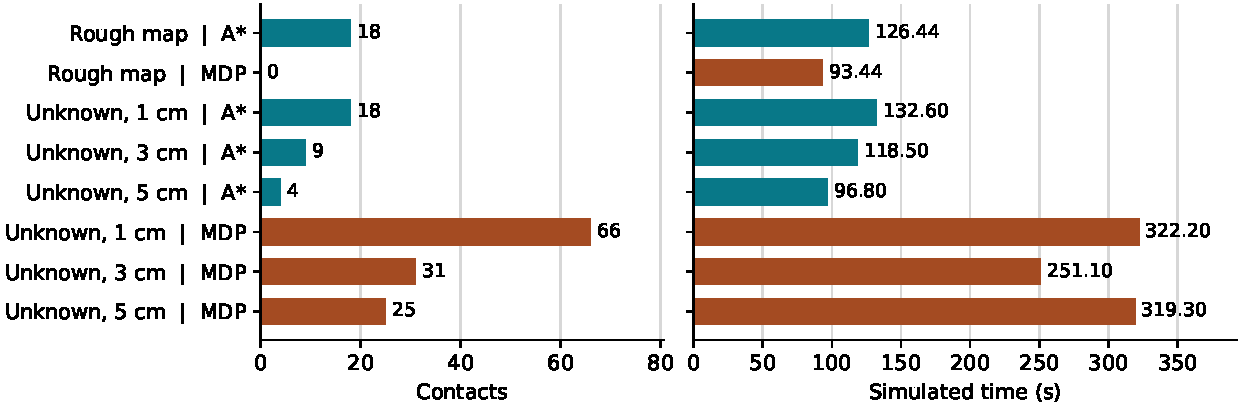
\includegraphics[width=.99\textwidth,height=.27\textheight,keepaspectratio]{strategy_metrics.pdf}
\caption{Total distance traveled including retreats, simulated time, and obstacle contacts for the single run of each strategy. In the unknown-box scenario, the step is the distance traveled along a box face between clearance checks.}
\label{fig:time}
\end{figure*}

\begin{figure*}[p]
\centering
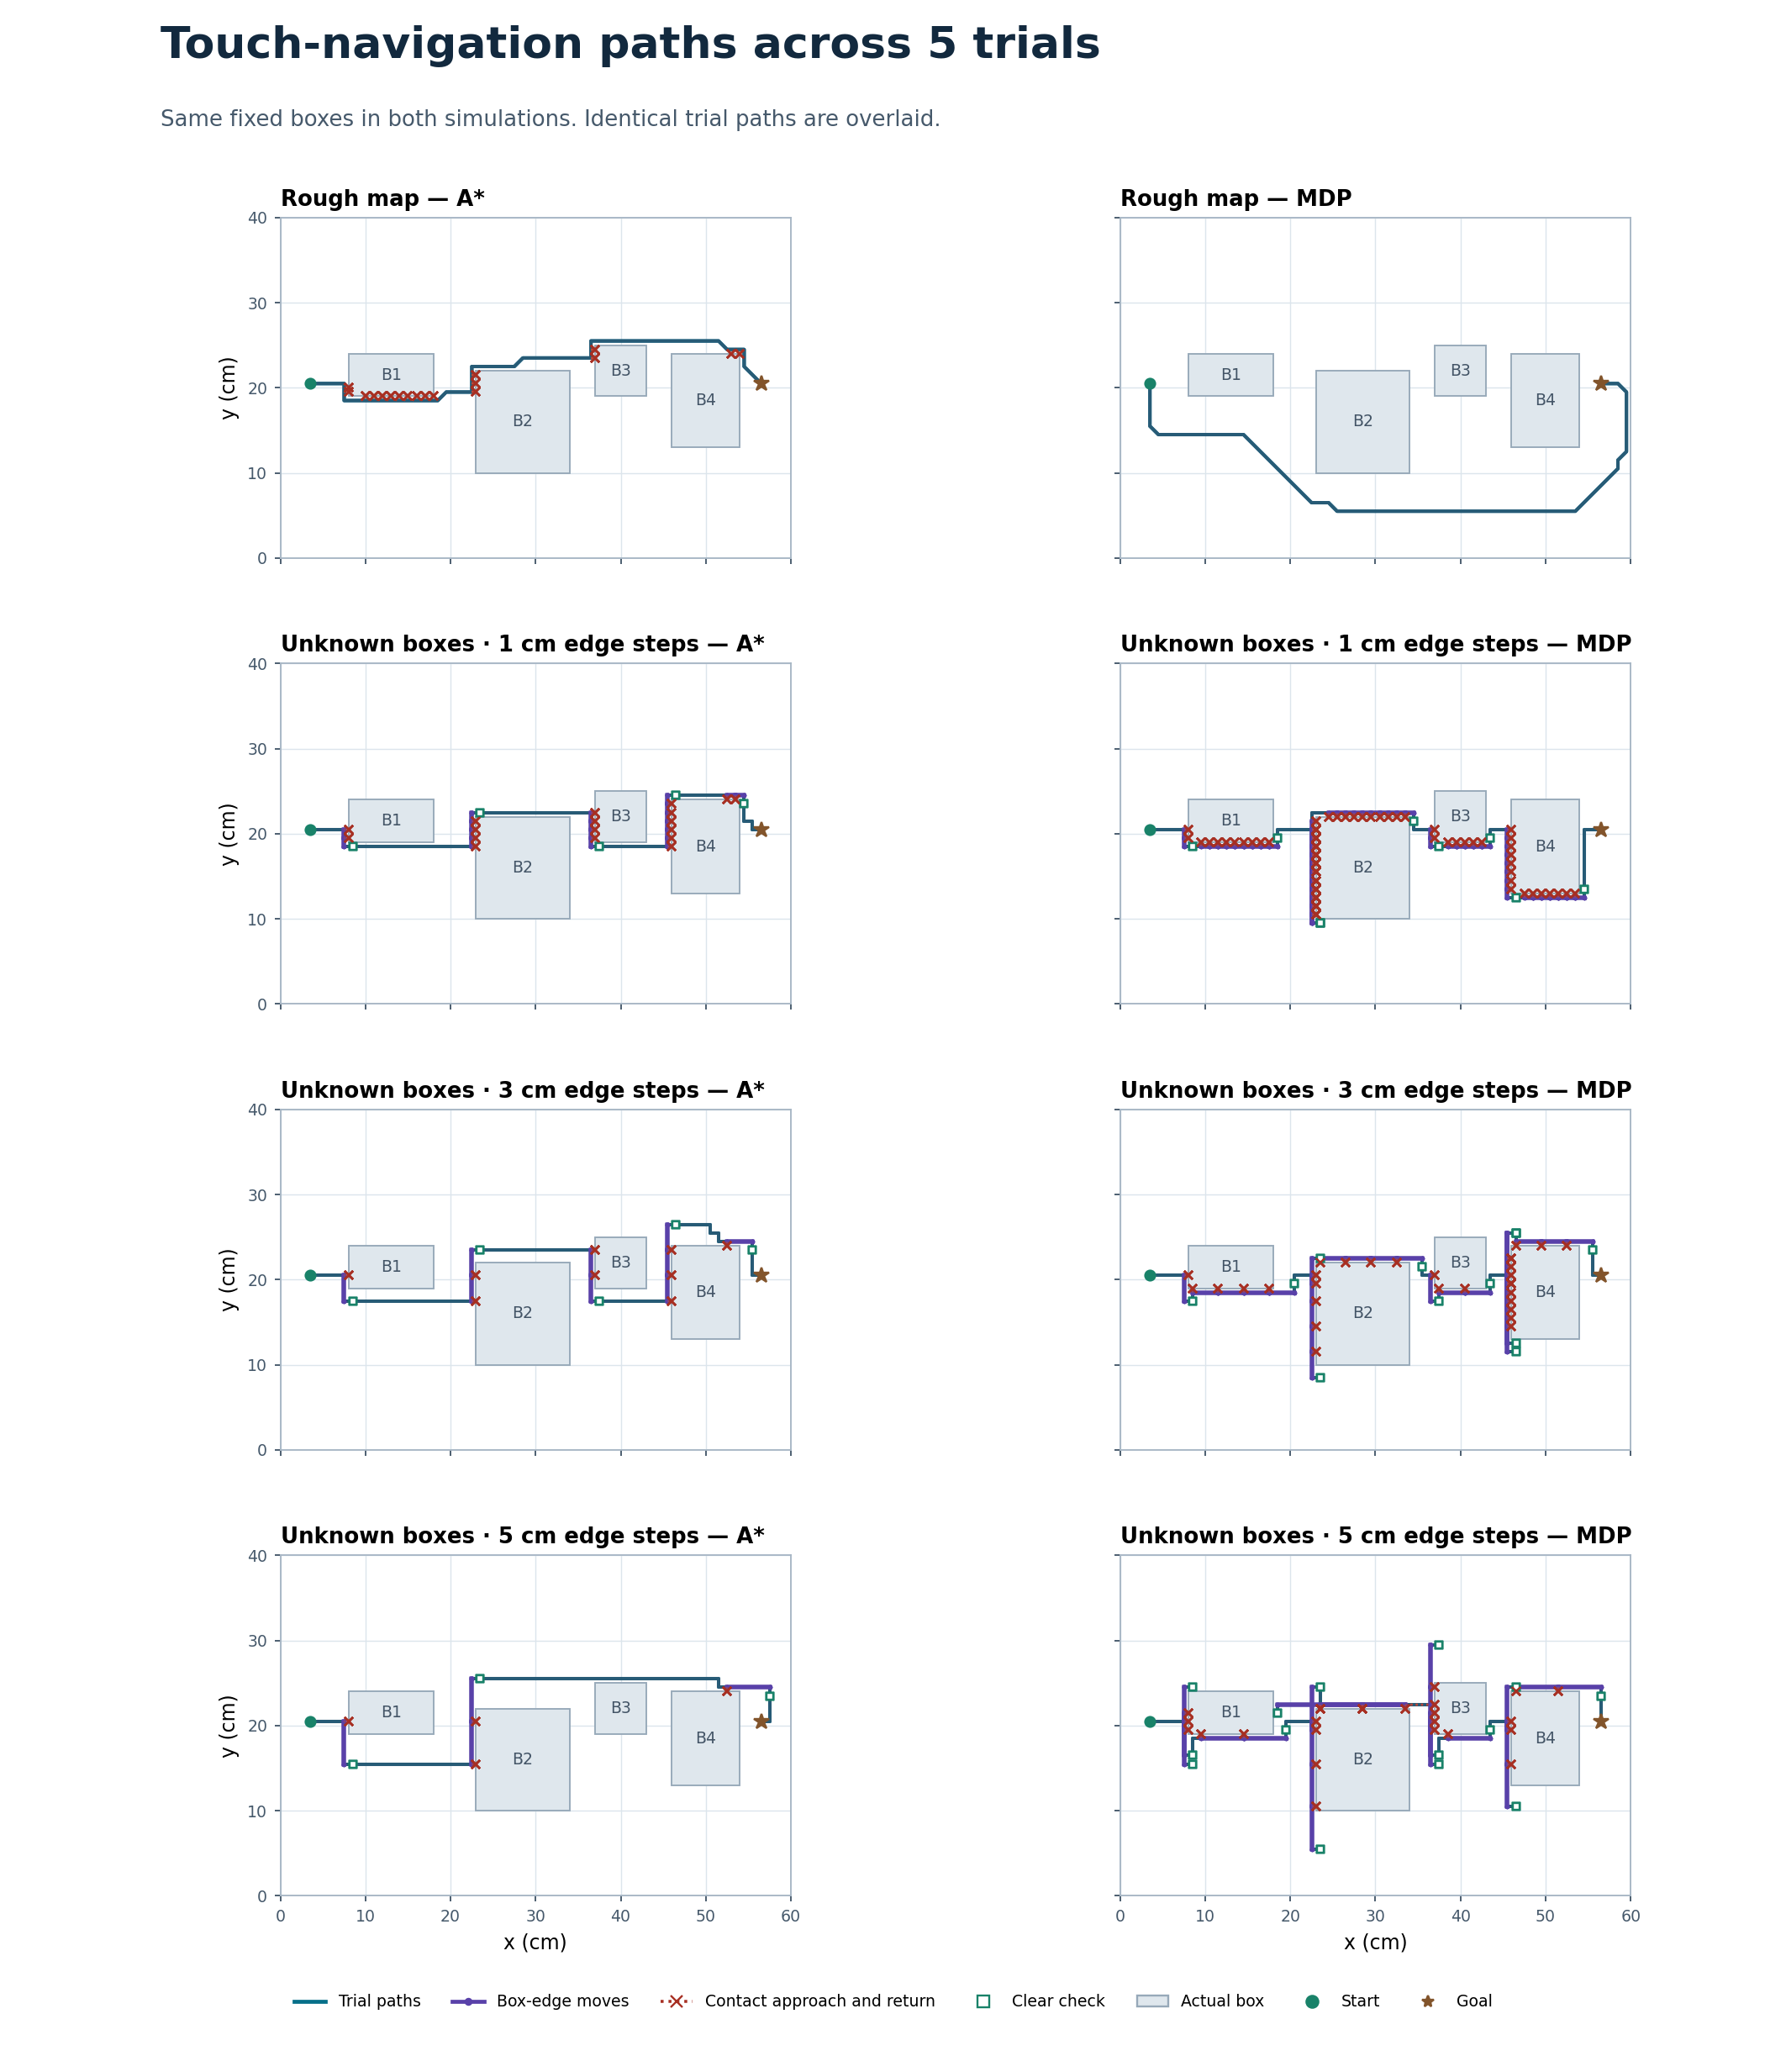
\includegraphics[width=.96\textwidth,height=.78\textheight,keepaspectratio]{simulation_paths.png}
\caption{The eight simulated paths. Purple segments mark box-face following. Red crosses mark contacts, and green squares mark successful clearance checks.}
\label{fig:paths}
\end{figure*}

\subsection{What the comparison covers}

The results describe one deterministic run per strategy on this box layout. Performance may change with a different layout or prior. The scenarios differ in both map information and allowed moves. For example, ordinary navigation allows diagonal moves only with the rough map. The simulator uses idealized grid readings for contact, and the reported times depend on the assumed motion and handling delays.

\section{UR5e Implementation and Reproducibility}

The robot script \texttt{ur5e\_runner.py} uses the same box-face routine as the simulator. It converts grid cells to robot target positions using the calibrated table frame. It uses force and pose readings to stop and retreat after contact and to estimate which cell the probe touched. The log records three phases: \texttt{navigate}, \texttt{edge\_follow}, and \texttt{edge\_check}.

The setup instructions use three grid cell centers to define the table frame. These are $(0,0)$, $(0,59)$, and $(39,0)$, taught at the trial height and orientation. The test plan uses the lab's approved motion and force settings. It starts with an empty table, then checks the 1, 3, and 5~cm steps with one secured box before the four-box trials. The probe starts each run stationary and unloaded at $(20,3)$, and each run has a separate log. The plan calls for one physical run per strategy. The planner has been checked offline with simulated observations. Physical trials and data collection are pending. Record physical run times separately from the simulated times in Table~\ref{tab:results}.

The \texttt{csv/} directory contains \texttt{trial\_results.csv} and \texttt{averages.csv}. With one run per strategy, each average equals the recorded trial value. From the project root, run \texttt{python run\_both\_simulations.py} to reproduce the CSV files and figures with Matplotlib.

\section{Conclusion}

The probe reached the goal in all eight simulation runs. With the rough map, the MDP reached the goal fastest and made no contacts. With unknown boxes, A* with a 5~cm step was fastest and made four contacts. For the MDP, a 3~cm step took less time than a 5~cm step. The longer step cut the number of contacts and increased the total distance traveled. Both measures help explain the time to reach the goal.

\bibliographystyle{IEEEtran}
\bibliography{references}

\end{document}
